\documentclass{beamer}
\usetheme{CambridgeUS} % replace it with Boadilla if you want no section bar
%\usecolortheme{crane} % other ones: dove, dolphin, rose, seahorse, orchid, crane, seagull, lily, wolverine
%\usefonttheme{serif} 
\usefonttheme[onlymath]{serif} % uncomment if you want it just for math

\setbeamertemplate{navigation symbols}{}  % comment to have nagivation

\usepackage[compress,comma,authoryear]{natbib}
\usepackage{tikz}
\usetikzlibrary{mindmap,trees}
\usepackage{amsmath,mathtools}
\usepackage{amsthm}
\usepackage{booktabs}
\usepackage{graphicx,epstopdf}
\usepackage{hyperref}


\definecolor{blue}{RGB}{0,114,178}
\definecolor{red}{RGB}{213,94,0}
\definecolor{yellow}{RGB}{240,228,66}
\definecolor{green}{RGB}{0,158,115}
\definecolor{Lblue}{RGB}{0,197,155}
\definecolor{Dblue}{RGB}{0,76,119}
\definecolor{Lgreen}{RGB}{180,255,230}

\hypersetup{
	colorlinks=false,
	linkbordercolor = {white},
	linkcolor = {blue}
}
\definecolor{MyBackground}{RGB}{245,245,245}

\setbeamercolor{frametitle}{fg=blue}
\setbeamercolor{title}{fg=blue}
\setbeamertemplate{footline}[frame number]
\setbeamertemplate{navigation symbols}{} 
\setbeamertemplate{itemize item}[circle]%{$\bigstar$}
\setbeamertemplate{itemize subitem}{$\bigstar$}
\setbeamercolor{itemize item}{fg=blue}
\setbeamercolor{itemize subitem}{fg=blue}
\setbeamercolor{enumerate item}{fg=blue}
\setbeamercolor{enumerate subitem}{fg=blue}
\setbeamercolor{button}{bg=MyBackground,fg=blue}
\setbeamercolor*{palette primary}{use=structure,fg=blue,bg=white}
\setbeamercolor*{palette secondary}{use=structure,fg=white,bg=Dblue}
\setbeamercolor*{palette tertiary}{use=structure,fg=white,bg=blue}
\setbeamercolor*{palette quaternary}{fg=white,bg=black}
\setbeamercolor*{palettes quaternary}{fg=white,bg=Lgreen}
%\setbeamercolor{titlelike}{parent=structure,bg=Lgreen}
%\setbeamercolor{title in head/foot}{bg=Lgreen,fg=orange}

\setbeamertemplate{enumerate item}{%
	\usebeamercolor[bg]{item projected}%
	\raisebox{1.5pt}{\colorbox{blue}{\color{fg}\footnotesize\insertenumlabel}}%
}


\begin{document}
	\title[Econometrics 2]{Econometrics 2 (M.Sc.)}
	\subtitle{Binary Choice Models}
	\author[Mohammad Hoseini]{Mohammad Hoseini}
	
	%\institute[IMPS]{Institute for Management and Planning Studies (IMPS)}
	
	\date[Spring 2024]{Spring 2024 \\
	\vspace{10pt} @metrics2
}
\begin{frame}[plain]
	\titlepage
\end{frame}

\section{Binary response models}

\begin{frame}{Binary variables}
A binary variable is one for observations that the event of interest has happened (success) and zero for the remaining observations (failure).
\begin{itemize}
	\item going to college
	\item owning a car
	\item having a job
\end{itemize}
\bigskip\pause

For binary variables, it is natural to think in terms of probabilities
\begin{itemize}
	\item What is the probability that an individual with characteristics $X$ goes to college
	\item If $X$ changes by one unit, how much does the probability change?
	
\end{itemize}
\end{frame}

\begin{frame}{Binary choice and probability}
With a random sample the sample mean of the binary variable is a good estimate of the unconditional probability that the event happens.
\[\Pr(y=1)=E[y]=\frac{1}{n}\sum_{i=1}^n y_i \]
What about conditional probability?\medskip

What factors do determine the change in the probability that $y$ equals one?\medskip\pause

Can we use linear regression for this?
\end{frame}


\begin{frame}{Linear probability model}
Consider $y=\beta_0+\beta_1x_1+\dots+\beta_kx_k+u=\mathbf{x\beta}+u$\bigskip

Assume that the residuals $u$ are uncorrelated with the regressors $\mathbf{x}$.\medskip
\[\Pr (y=1|\mathbf{x})=E(y=1|\mathbf{x})=\mathbf{x\beta} \text{ and } \Pr (y=0|\mathbf{x})=1-\mathbf{x\beta}\]
This is called the \textbf{linear probability model} because the probability of success (i.e. $y = 1$) is a \textbf{linear} function of the explanatory variables.\bigskip\medskip

Because the model is linear, change in the probability of success, resulting from a change in $x_j$, holding other factors constant becomes:
\[\Delta \Pr(y=1|\mathbf{x})=\beta_j\Delta x_j \]

\end{frame}

\begin{frame}{Shortcoming of linear probability model (LPM)}
There is no guarantee that the values of $\mathbf{x\beta}$ lies between 0 and 1.\bigskip

A probability cannot be \textbf{linearly} related to all possible values of a continuous variable.
\begin{itemize}
\item ``An increase in wealth by 1 unit increases the probability of owning car by 1 percent'' is reasonable statement for a person with average wealth level.
\item LPM gives reasonable estimates of partial effects only near the center of the distribution of $\mathbf{x\beta}$.
\item For extreme values close to 0 or 1, using LPM doesn't make sense.
\end{itemize}
\end{frame}

\begin{frame}{Shortcoming of linear probability model (LPM)}
In LPM, the residuals are heteroskedastic and depend on $\mathbf{x}$:
\[ \text{var}(u|\mathbf{x})=\Pr(y=1|\mathbf{x})(1-\mathbf{x\beta})^2+\Pr(y=0|\mathbf{x})(-\mathbf{x\beta})^2 \]
\[\qquad= \mathbf{x\beta}(1-\mathbf{x\beta})^2+(1-\mathbf{x\beta})(-\mathbf{x\beta})^2= \mathbf{x\beta}(1-\mathbf{x\beta})\]
what can we do for this? \pause  
robust standard errors \bigskip

Another problem in LPM is that the residuals are not normally distributed and inference on small sample cannot be based on a t-test.
\end{frame}

\begin{frame}{Nonlinear probability model}
To solve the problems of linear probability model consider
\[\Pr(y=1|\mathbf{x})=F(\beta_0+\beta_1x_1+\dots+\beta_kx_k)=F(\mathbf{x\beta}) \]
where for all real numbers $0<F(.)<1$. Now we ensure that the estimated probability lies between 0 and 1.\bigskip

What function can we use for $F(.)$?\pause\medskip

$F$ is normally a cumulative density function which is increasing in $\mathbf{x\beta}$:
\[\Pr_{\mathbf{x\beta}\rightarrow+\infty}(y=1|\mathbf{x})=F(+\infty)=1\qquad \Pr_{\mathbf{x\beta}\rightarrow-\infty}(y=1|\mathbf{x})=F(-\infty)=0   \]
As $F(.)$ is non-linear, we cannot use OLS.

\end{frame}

\begin{frame}{Logistic and Normal distributions}
Various CDF functions for $F$ have been suggested in the literature. \medskip

By far the most common ones are the \textbf{logistic} distribution and the \textbf{normal} distribution.

\begin{center}
\begin{tikzpicture}
\draw[->] (-4.5,0) -- (4.5,0) node[right] {$x$};
\draw[->] (0,0) -- (0,3) node[above] {$f(x)$};
\draw[scale=1,domain=-4:4,smooth,variable=\x,blue] plot ({\x},{5*exp(-\x*\x/2)/2.5066282}) node[below] {normal};

\draw[scale=1,domain=-2.5:2.5,smooth,variable=\x,red]  plot ({\x},{5*exp(-\x /0.551328)/(0.551328*(1+exp(-\x /0.551328))*(1+exp(-\x / 0.551328)))}) node[above] {logistic};
\end{tikzpicture}
\end{center}

\end{frame}
\begin{frame}{Logit model}
Logistic distribution:
\[ f(z)=\frac{1}{(\exp^{-z/2}+\exp^{z/2})^2}\qquad F(z)=\frac{\exp(z)}{1+\exp(z)} \]\bigskip

The \textbf{logit} model:\[\Pr(y=1|\mathbf{x})=\frac{\exp(\mathbf{x\beta})}{1+\exp(\mathbf{x\beta})} \]
\end{frame}

\begin{frame}{Probit model}
Normal distribution:
\[f(z)=\frac{1}{\sqrt{2\pi}}\exp(-z^2/2)\qquad F(z)=\int_{-\infty}^{z}f(t)dt \]
\bigskip

The \textbf{probit} model:\[\Pr(y=1|\mathbf{x})=\int_{-\infty}^{\mathbf{x\beta}}\frac{1}{\sqrt{2\pi}}\exp(-t^2/2)dt \]

\end{frame}

\begin{frame}{ML estimation of logit and probit}
\[\text{The assumption is } \Pr (y=1|\mathbf{x})=F(\mathbf{x\beta})  \text{ and } \Pr (y=0|\mathbf{x})=1-F(\mathbf{x\beta}) \]
Likelihood function:\[L(y|x,\beta)=\prod_{y_i=0}\big(1-F(\mathbf{x}_i\beta)\big) \prod_{y_i=1}F(\mathbf{x}_i\beta) \]
\[L(y|x,\beta)=\prod_{i=1}^nF(\mathbf{x_i\beta})^{y_i}\big(1-F(\mathbf{x_i\beta})\big)^{1-y_i}  \]
Log-likelihood function:
\[LL(y|x,\beta)=\sum_{i=1}^n y_i\ln F(\mathbf{x}_i\beta)+(1-y_i)\ln(1-F(\mathbf{x}_i\beta)) \]

\end{frame}

\begin{frame}{LL of logit and probit}
\[LL(y|x,\beta)=\sum_{i=1}^n y_i\ln F(\mathbf{x}_i\beta)+(1-y_i)\ln(1-F(\mathbf{x}_i\beta)) \]
Logit: \[LL(y|x,\beta)=\sum_{i=1}^n y_i\ln \Big(\frac{\exp(\mathbf{x}_i\beta)}{1+\exp(\mathbf{x}_i\beta)} \Big)+(1-y_i)\ln \Big(\frac{1}{1+\exp(\mathbf{x}_i\beta)} \Big) \]
\[LL(y|x,\beta)=\sum_{i=1}^n y_i \mathbf{x}_i\beta-\ln\Big(1+\exp(\mathbf{x}_i\beta)\Big) \]
Probit ($\Phi$ is the standard normal CDF function): \[LL(y|x,\beta)=\sum_{i=1}^n y_i\ln \Phi(\mathbf{x}_i\beta)+(1-y_i)\ln(1-\Phi(\mathbf{x}_i\beta)) \]
\end{frame}

\begin{frame}{Goodness to fit in logit and probit}
Recall in linear regression $R^2=\frac{\text{var}(\hat{y})}{\text{var}(y)}$ measures the goodness of fit.\medskip

In nonlinear models we can't use simple $R^2$, but there are different alternatives. The most common one is \textbf{Pseudo R-squared}
\[ \tilde{R}^2=1-\frac{LL(\text{model with predictors } \mathbf{x})}{LL(\text{model with only an intercept})} \] \medskip
Note that as $0<L<1$, we have $-\infty<LL<0$.
\begin{itemize}
\item If the independent variables have no explanatory power at all, then the fraction is one and we get $\tilde{R}^2 = 0$.
\item If the independent variables are doing well, then the $LL$ value in numerator approaches 0 and we get $\tilde{R}^2 = 1$.
\end{itemize}
\end{frame}

\begin{frame}{Interpretation }
The logit and probit functions are both increase relatively quickly at $\mathbf{x\beta}=0$, while the effect on $F$ at extreme values of $\mathbf{x\beta}$ tends to zero.\medskip

This result ensures that the marginal effects of changes in $x_j$ is not constant, a concern we had with the LPM.\medskip

Interpretation of logit and probit is less straightforward than LPM.\bigskip

In LPM marginal effect of change in $x_j$ is simply $\displaystyle\frac{\Delta \Pr(y=1|\mathbf{x})}{\Delta x_j}=\beta_j$ \bigskip


What is the marginal effect in logit and probit?
\end{frame}

\begin{frame}{Marginal effect}
for logit and probit models obtaining measures of the marginal effect is more complicated. \bigskip

When $x_j$ is a continuous variable, its marginal effect on $\Pr (y = 1|x)$ is obtained from the partial derivative:
\[\frac{\partial \Pr (y=1|x)}{\partial x_j}=\frac{\partial F(\mathbf{x\beta})}{\partial x_j}=\beta_j.f(\mathbf{x\beta}) \]
Because the density function is non-negative, the marginal effect of $x_j$ will always have the same sign as $j$.\bigskip

Therefore, knowing the sign of $\beta_j$ is sufficient for determining whether the effect is positive or negative, but to find the magnitude of the effect we have to use the formula above.
\end{frame}

\begin{frame}{Marginal effect of continuous variables}
The marginal effect depends on $f(\mathbf{x\beta})$ and for different values of $x_1,\dots, x_k$ the marginal effect will be different.\bigskip 

\textbf{Marginal effect at sample mean}: One possibility is to evaluate marginal effects at the sample mean values of $x_1,\dots, x_k$.\bigskip

\textbf{Average marginal effect}: Alternatively, we can compute marginal effects for each observation in the sample and average them.\bigskip

\textbf{Marginal effect at a point}: Also, based on the problem at hand, we can compute them at a specific point. Suppose $x$ is income and we are interested in marginal effect of the poor.

\end{frame}

\begin{frame}{Marginal effect of discrete variables}
When an explanatory variable is discrete, consider two values and find the marginal effect as the difference.\bigskip 

For example, assume $x_1$ is gender (0=male, 1=female), then the marginal effect of changing gender from male to female, while holding all other variables fixed, is
\[F(\beta_0+\beta_1\times 1+\dots+\beta_kx_k)-F(\beta_0+\beta_1\times 0+\dots+\beta_kx_k) \]
Depending where we want to estimate the marginal effect  (sample mean, average effect, or a specific point), we set the values of the rest of explanatory variables $x_2,\dots,x_k$.
\end{frame}

\begin{frame}{Latent variable model}
The traditional view to probits and logits in econometrics is based on \textbf{latent variable model} in which the dependent variable is unobserved.\bigskip

Let $y^*$ be a continuous variable that we do not observe (latent variable) and assume 
\[y^* =\beta_0+\beta_1x_1 +\beta_2x_2 + \dots + \beta_Kx_K + e=\mathbf{x\beta}+e  \]
While we do not observe $y^*$, we do observe the discrete choice made by the individual, according to the following choice rule:
\[y = 1 \text{ if } y^*> 0 \qquad y = 0 \text{ if } y^* \le 0\]
Think about $y^*$ as the net utility of a choice considering the cost and benefits. If the utility is positive the choice is made otherwise not.
\end{frame}

\begin{frame}{Latent variable model}
\[y^* =\mathbf{x\beta}+e \qquad y = 1 \text{ if } y^*> 0 \qquad y = 0 \text{ if } y^* \le 0 \]\bigskip

Assume the error terms have distribution $f(z)$ which is \textbf{symmetric}
\[\Pr(y=1|x)=\Pr(y^*>0|x)=\Pr(\mathbf{x\beta}+e>0|x)=\Pr(e>-\mathbf{x\beta}) \]
\[= 1-F(-\mathbf{x\beta})=F(\mathbf{x\beta}) \]

The last step exploit the symmetry property. As both normal and logistic distributions are symmetric, we can derive probit and logit models based on this method too.
\end{frame}

\begin{frame}{Logit vs. probit}
Logit and probit are models. ``All models are wrong, some are useful''.\bigskip

Probit is more natural when we think of a latent variable model.\bigskip

Logit can be interpreted as modeling log odds (odds ratio).\bigskip 

Logit is simpler to estimate and much faster in large samples. This is because to find $\Pr(y=1|\mathbf{x})$ numerical integration is needed in probit, but not in logit.\bigskip

Usually people start with logit. \bigskip

We can also use likelihood value to decide logit or probit.

\end{frame}


%\begin{frame}{LPM vs logit/probit}
%	\begin{figure}
%		\centering
%		
\includegraphics[width=0.9\linewidth]{../figure/lpmtwit}
%	\end{figure}
%\end{frame}
%
\begin{frame}{Fractional outcome}
In many cases the outcome variable is proportional (Gini coefficient, unemployment rate, \dots)\bigskip

In this circumstances, the outcome is not binary but lies between [0,1]\bigskip

It is like that instead of either 0 or 1, you have probabilities that are continuous.\bigskip

For continuous variables, we normally use OLS and here we can too.\bigskip

But as we saw for LPM, if we do that the predictions could fall outside [0,1].
\end{frame}

\begin{frame}{Fractional response model}
Fractional response models make a similar assumption as binary choice models:
\[y_i=F(\beta_0+\beta_1x_{1i}+\dots+\beta_kx_{ki})+\varepsilon_i \]
Where common distributions used for $F(.)$ are of normal, logistics, and beta.\bigskip

Estimation is by MLL method and in STATA use can use \texttt{fracreg}. \bigskip

Shall we always use fractional response estimation with proportional variables?
\begin{itemize}
\item Not really. Again it depends on the data.
\end{itemize}

\end{frame}

\begin{frame}{Fractional Response vs. OLS}

If the proportional variable has a concentrated distribution similar to Normal, OLS is ok and even more efficient.\medskip

But if the variable's distribution looks more like Bernoulli than Normal you should use fractional response.

\begin{center}
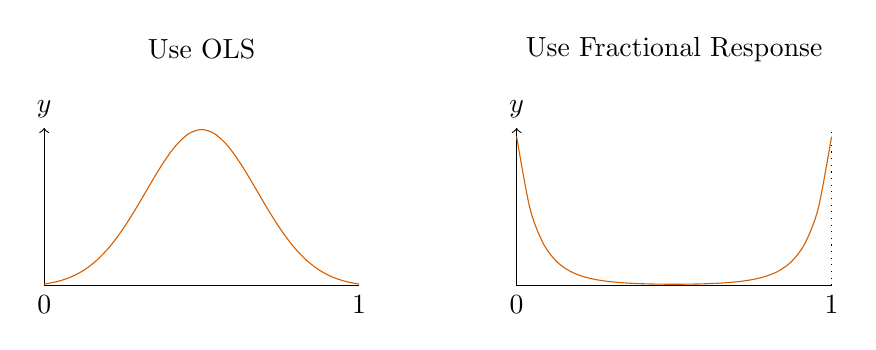
\begin{tikzpicture}
\draw[<-] (-5,2) node[above] {$y$} -- (-5,0) node[below ] {$0$} -- (-1,0) node[below] {$1$};
\draw[<-] (1,2) node[above] {$y$} --(1,0) node[below] {$0$} -- (5,0) node[below] {$1$};
\draw[dotted] (5,0) -- (5,2);
\draw (-3,3) node {Use OLS};	\draw (3,3) node {Use Fractional Response};
\draw[scale=1,domain=-5:-1,smooth,variable=\x,red]  plot ({\x},{2*exp(-(\x+3)*(\x+3))-.02});	\draw[scale=1,domain=1:5,smooth,variable=\x,red]  plot ({\x},{.035*exp((\x-3)*(\x-3))-.02});
\end{tikzpicture}
\end{center}

\end{frame}


%\begin{frame}{References:}
%\bibliographystyle{apalike}
%\small
%\bibliography{references}
%\end{frame}

\end{document}
